\lstinputlisting[language=bash,basicstyle=\small]{python_codes/fieldstone_93/keywords}

\begin{center}
Code at \url{https://github.com/cedrict/fieldstone/tree/master/python_codes/fieldstone_93}
\end{center}

\par\noindent\rule{\textwidth}{0.4pt}

%%%%%%%%%%%%%%%%%%%%%%%%%%%%%%%%%%%%%%%%%%%%%%%%%%%%%%%%%%%%%%%%%%%%%%%%%%%%%%%%%%%%%%%%%%%%%%%%%%%%


This stone solves the problem of the Stokes sphere sinking under a deformable free surface, 
It relies on an unstructured grid with Crouzeix-Raviart elements (see Section~\ref{ss:XXX}).

The workflow is as follows: the main parameters are defined in {\sl parameters.py}.
The file {\sl generate\_nodes.py} uses these parameters to generate points on the 
boundary of the rectangular domain, on the surface and on the circle and its center. 
A call to {\sl triangle} is then made and a very important additional parameter is passed
as argument to triangle: the maximum area of a triangle. 
{\sl triangle} returns the (constrained) Delaunay triangulation of these points, 
and this information is then read in by {\sl stone.py} which solves the 
Stokes equation. 
Boundary conditions are free slip everywhere. This benchmark is described in 
Section~\ref{ss:stokes_sphere_fs2D}.

All these actions are carried out automatically when the following script is 
used\footnote{It assumes that the triangle program has been compiled and 
is located outside of the fieldstone tree.}:
\begin{lstlisting}
python3 generate_nodes.py
cat mypoints mysegments > mesh.poly
../../../../triangle/triangle  -j -q -a0.00100 -o2 -pc mesh.poly
echo "nel="
head -1 mesh.1.ele 
head -1 mesh.1.ele > temp
echo "NV0="
head -1 mesh.1.node 
head -1 mesh.1.node >> temp
python3 stone.py
\end{lstlisting}


Note that ressure normalisation is not done the right way: the pressure nullspace is 
not removed from the matrix, but the solution is later normalised at the top
of the domain so that its average over the domain is zero.

Time stepping is carried out and the time step $\delta t$ is computed with a CFL criterion.
Nodes are advected with their velocity but no remeshing is implemented so that when the 
deformation becomes to large around the sphere the triangles become really deformed and 
the simulation must be stopped. Given the parameters of this benchmark this corresponds 
to $t\simeq 30$, while the simulation should ideally have been run up to $t>100$.

Nodes on the deformable surface are flagged at the beginning of the calculations and 
exported to an ascii file for later postprocessing. The multiple measurements for this 
benchmark are thoroughly described and plotted in Section~\ref{ss:stokes_sphere_fs2D}.


\begin{center}
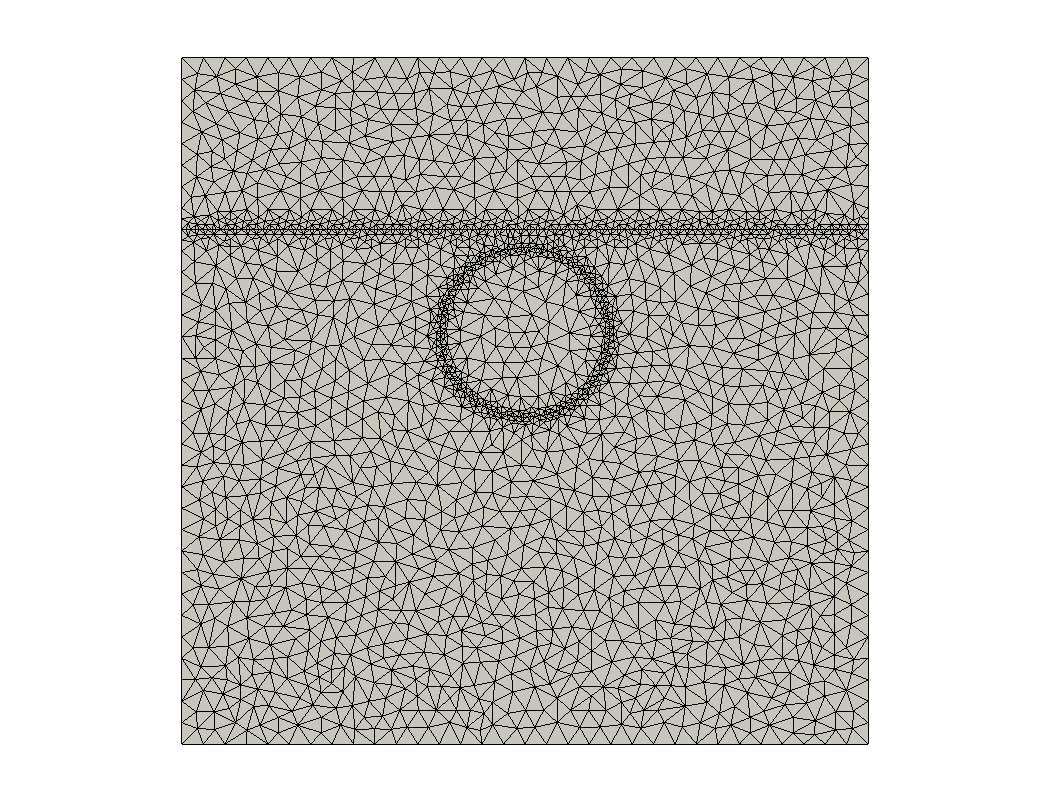
\includegraphics[width=6.5cm]{python_codes/fieldstone_93/50/mesh0000}
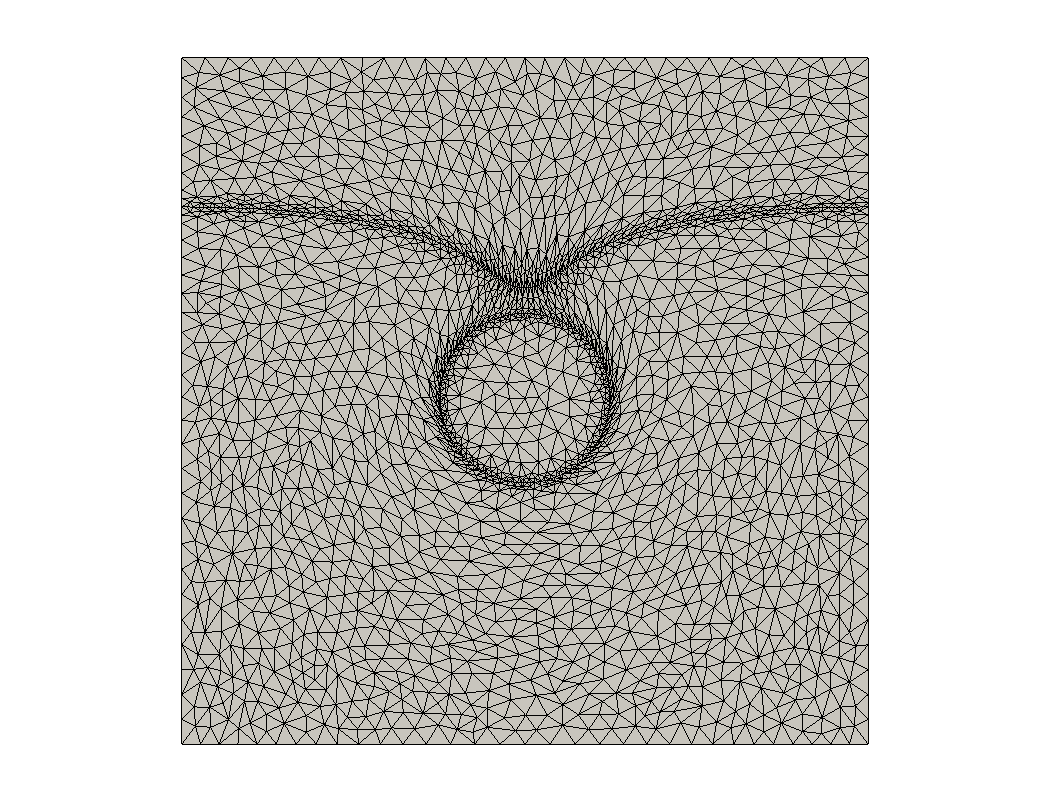
\includegraphics[width=6.5cm]{python_codes/fieldstone_93/50/mesh0136}\\
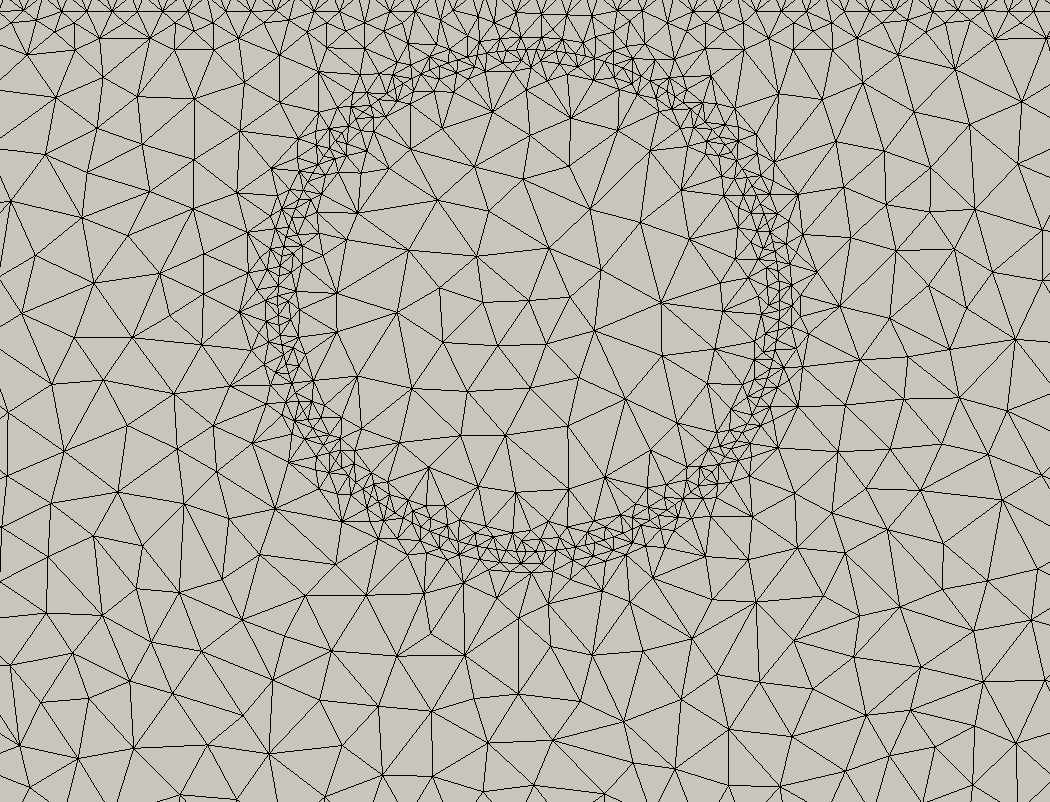
\includegraphics[width=5.5cm]{python_codes/fieldstone_93/50/meshzoom0000}
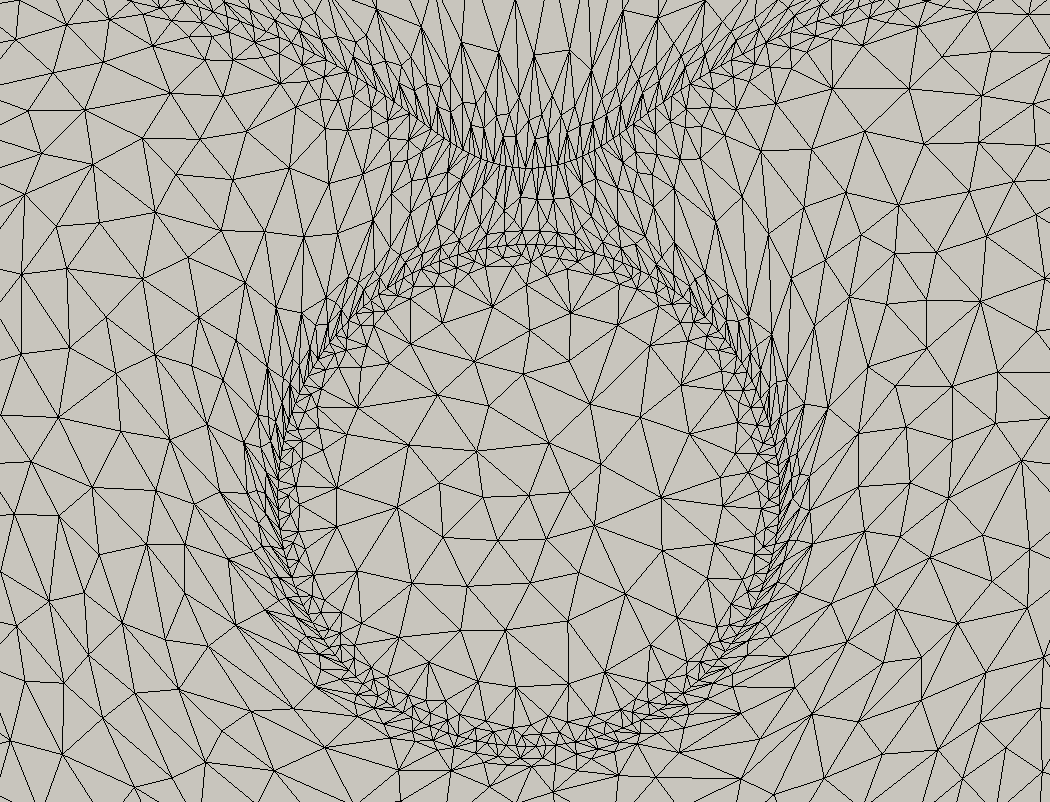
\includegraphics[width=5.5cm]{python_codes/fieldstone_93/50/meshzoom0136}\\
{\captionfont  Mesh obtained with -a0.00050 in script}
\end{center}

\begin{center}
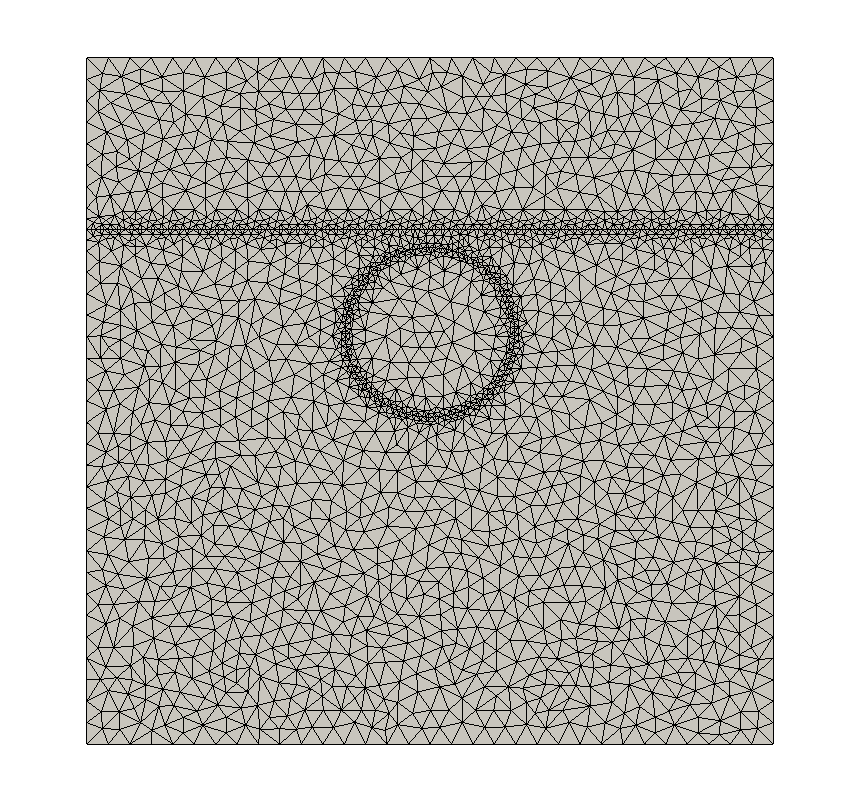
\includegraphics[width=5.5cm]{python_codes/fieldstone_93/results/mesh1}
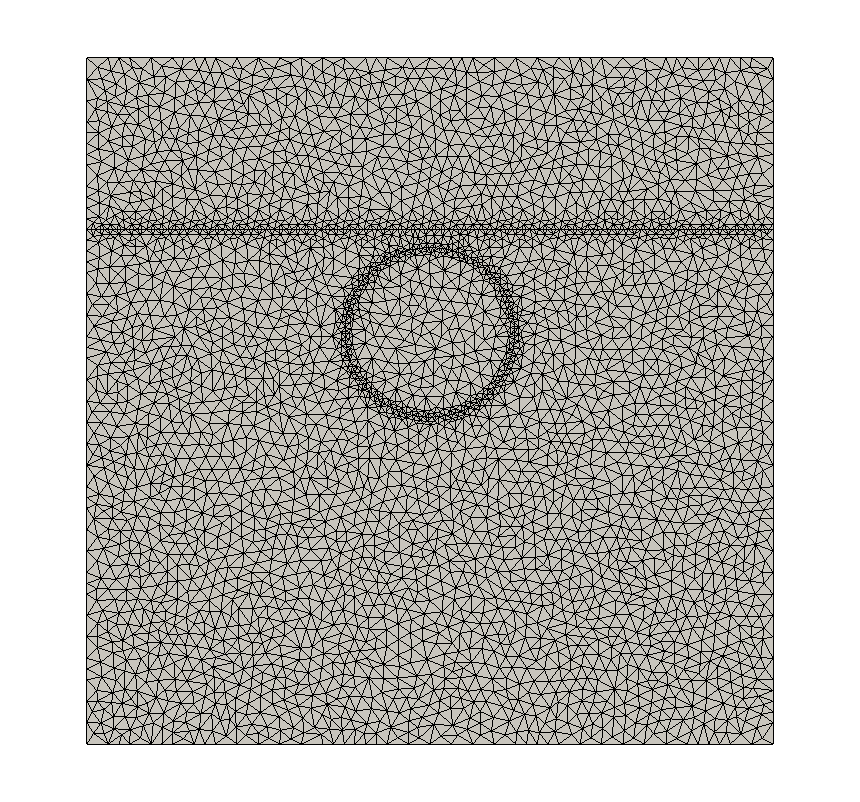
\includegraphics[width=5.5cm]{python_codes/fieldstone_93/results/mesh2}
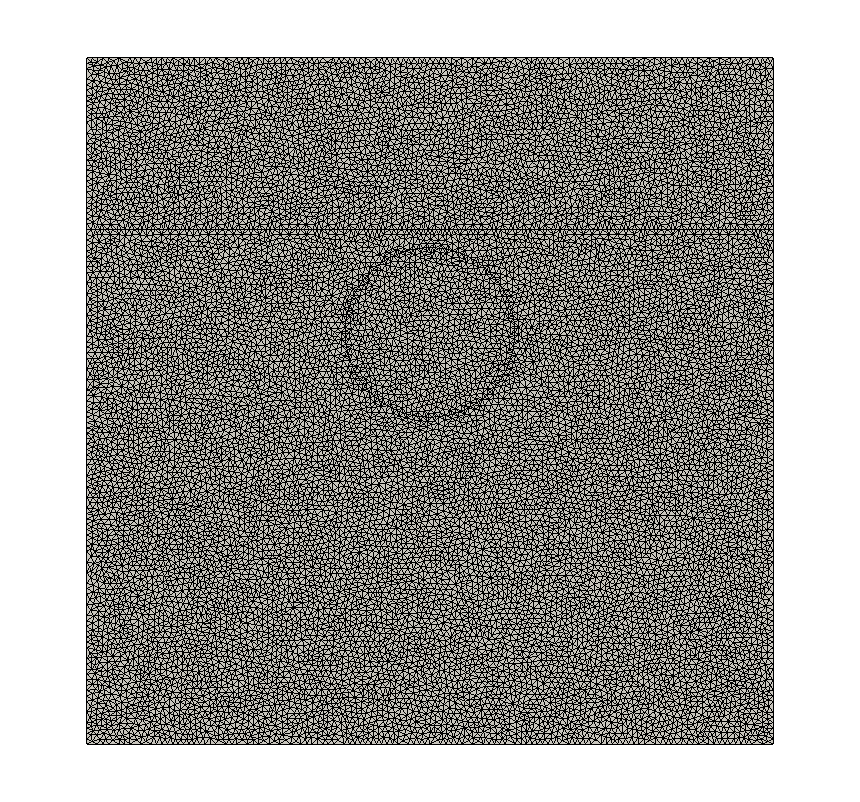
\includegraphics[width=5.5cm]{python_codes/fieldstone_93/results/mesh3}\\
{\captionfont  Mesh obtained with -a0.00050, -a0.00025 and -a0.00005 in script}
\end{center}

\begin{center}
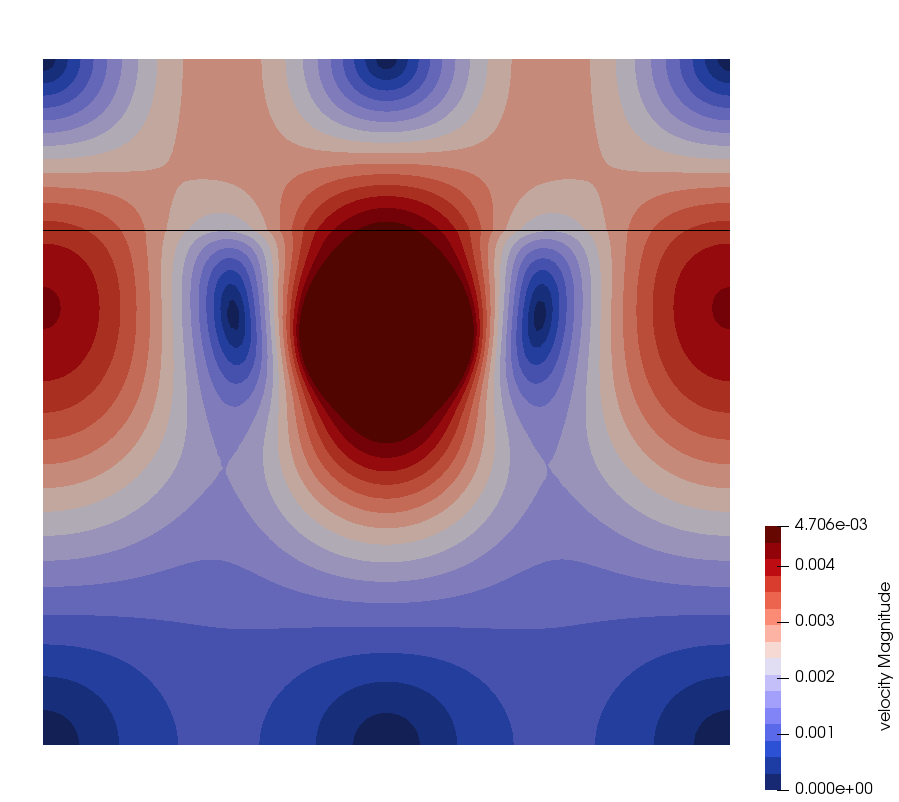
\includegraphics[width=4cm]{python_codes/fieldstone_93/results/vel_0000}
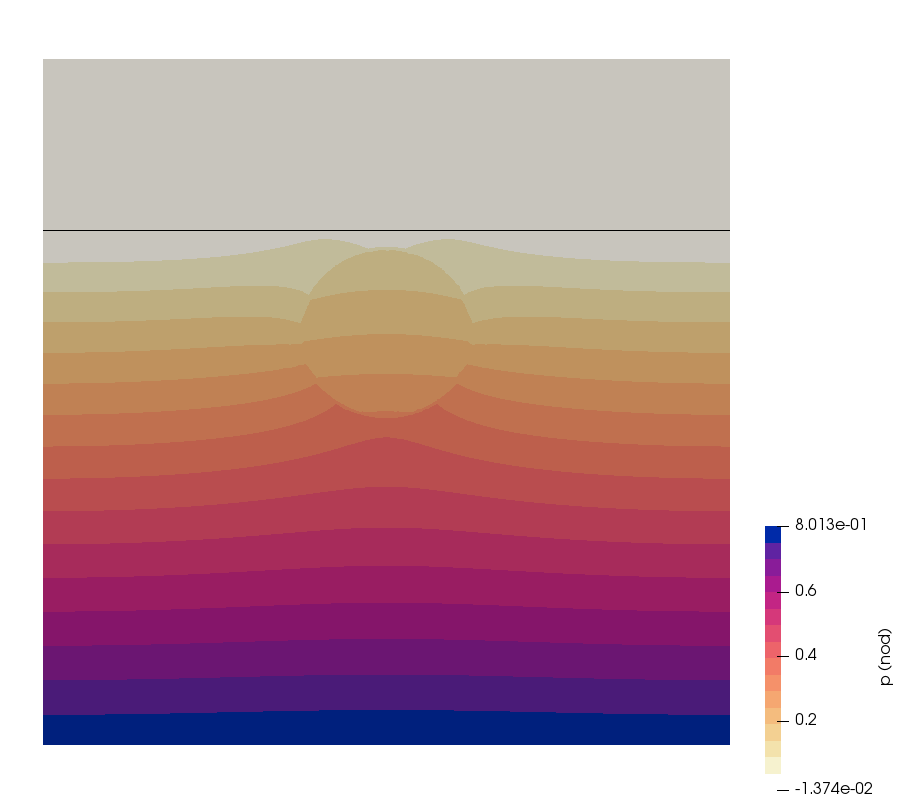
\includegraphics[width=4cm]{python_codes/fieldstone_93/results/p_0000}
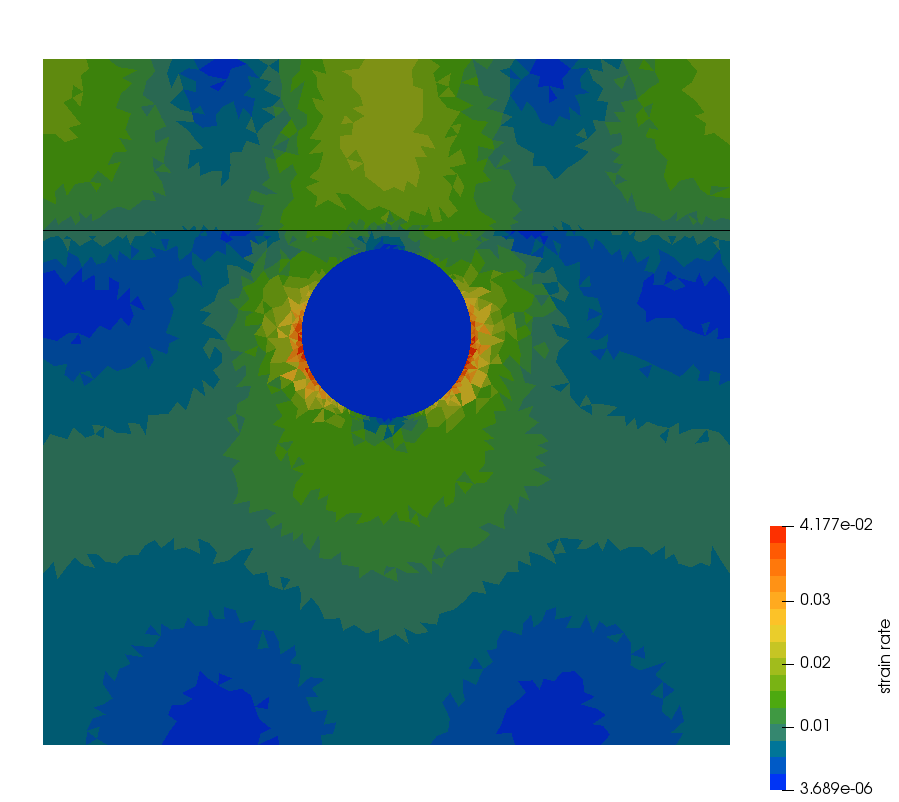
\includegraphics[width=4cm]{python_codes/fieldstone_93/results/sr_0000}
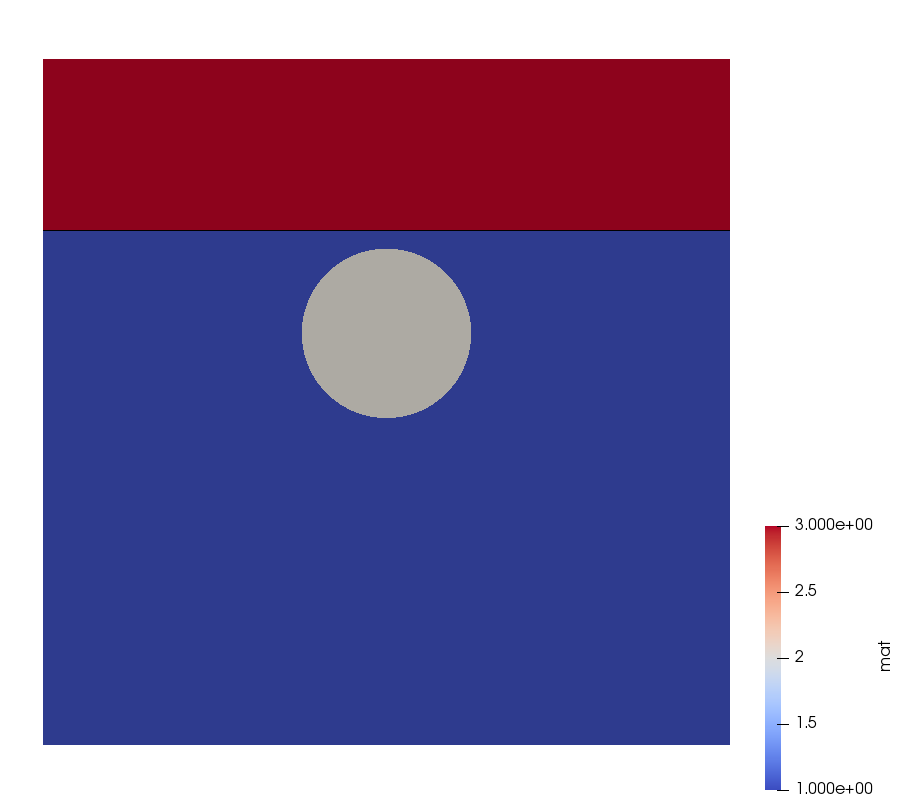
\includegraphics[width=4cm]{python_codes/fieldstone_93/results/mat_0000}\\
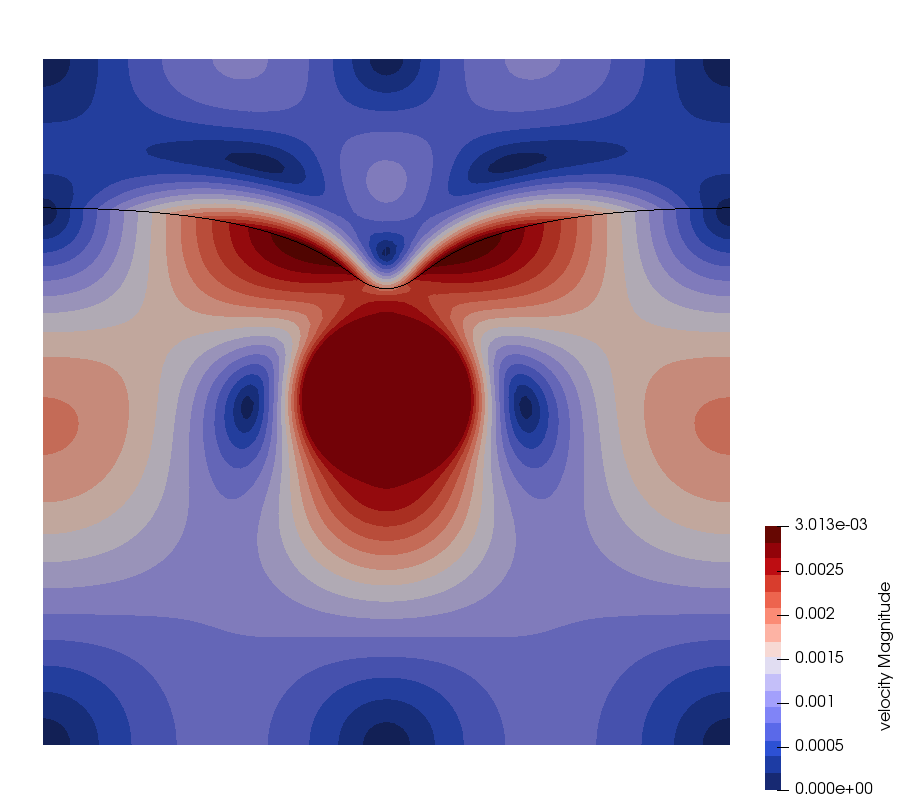
\includegraphics[width=4cm]{python_codes/fieldstone_93/results/vel_0136}
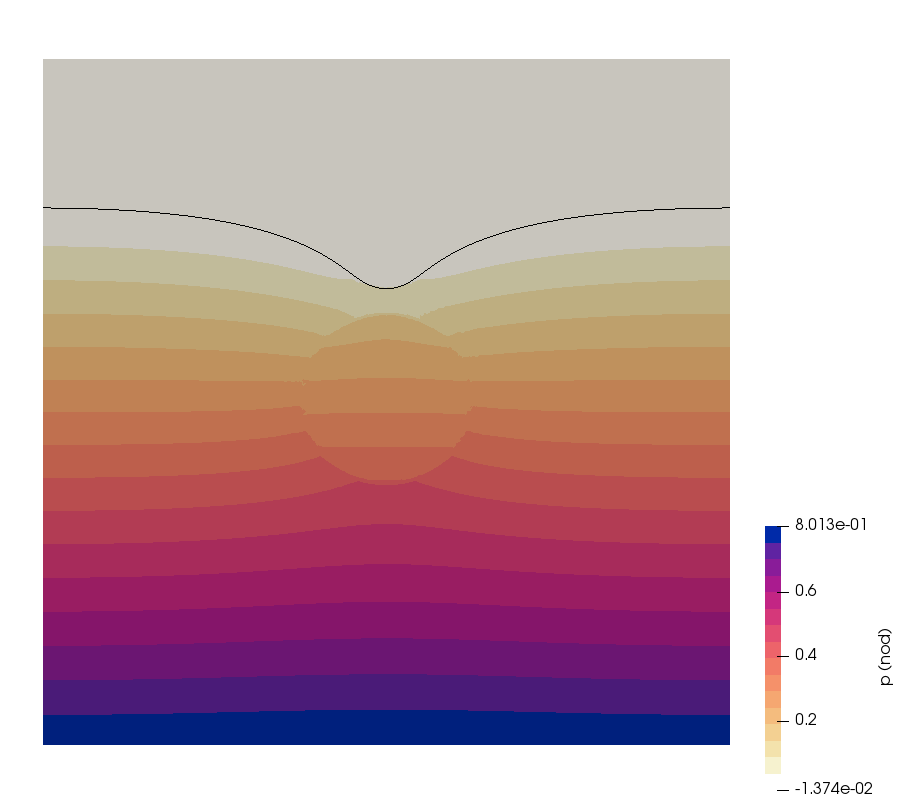
\includegraphics[width=4cm]{python_codes/fieldstone_93/results/p_0136}
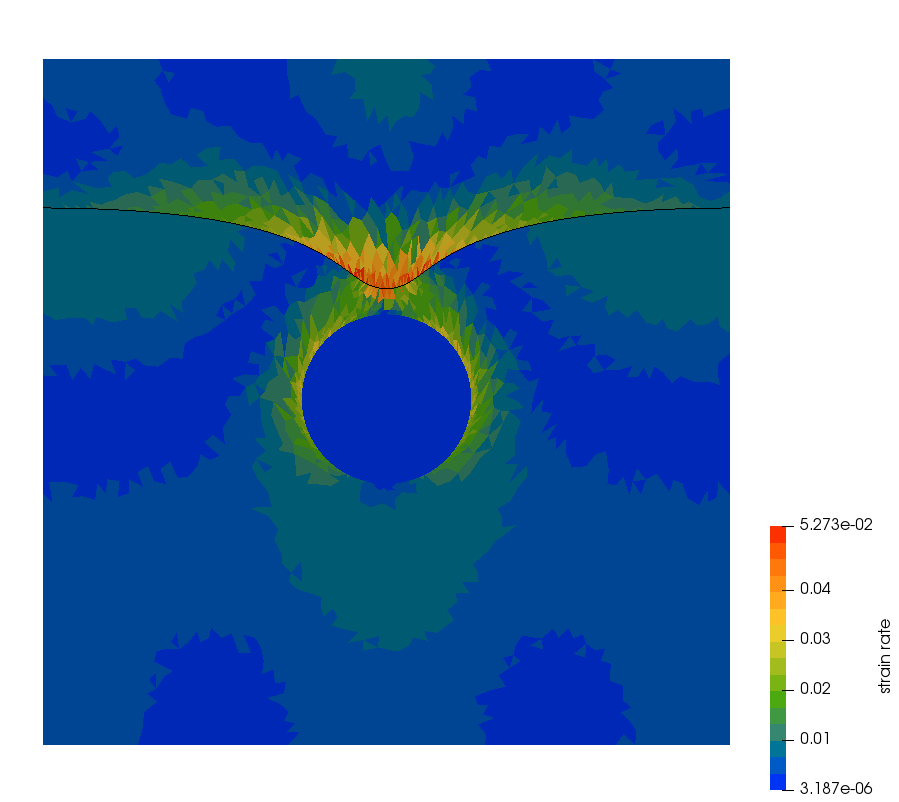
\includegraphics[width=4cm]{python_codes/fieldstone_93/results/sr_0136}
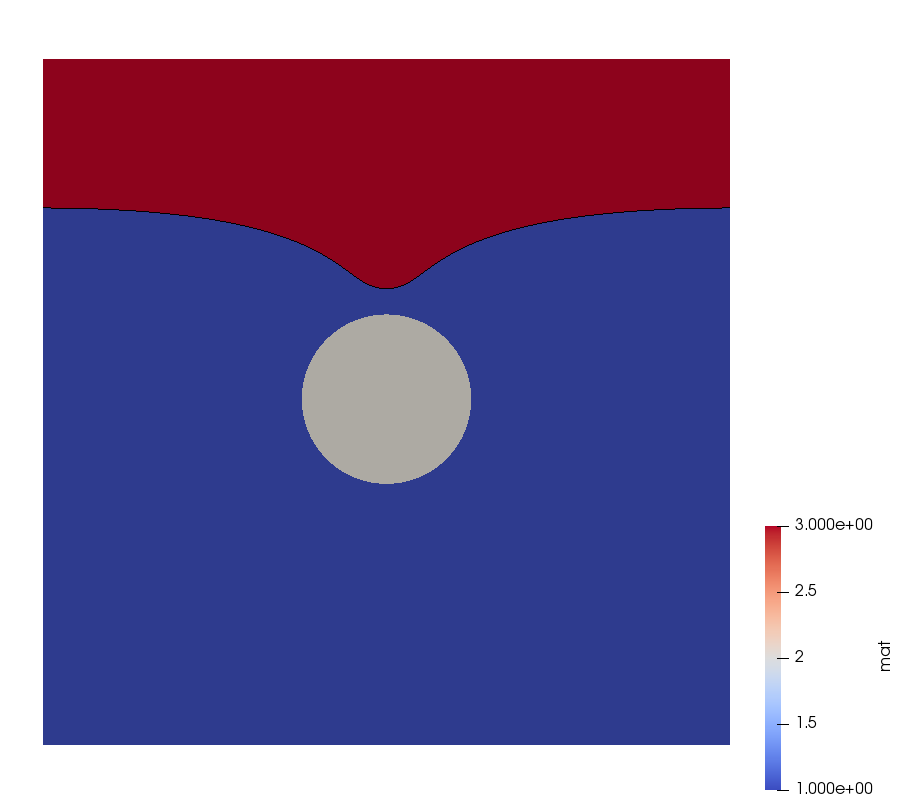
\includegraphics[width=4cm]{python_codes/fieldstone_93/results/mat_0136}\\
{\captionfont  Mesh obtained with -a0.00025 in script. Top row $t=0$, 
bottom row $t\simeq 30$.}
\end{center}


\newpage

\begin{center}
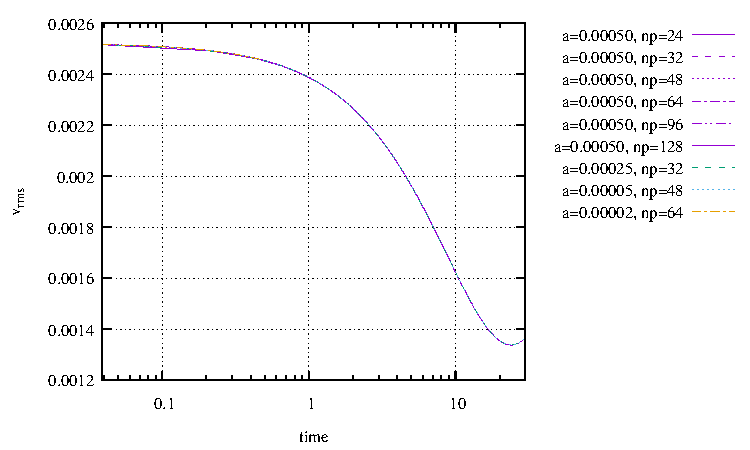
\includegraphics[width=5.7cm]{python_codes/fieldstone_93/results/vrms}
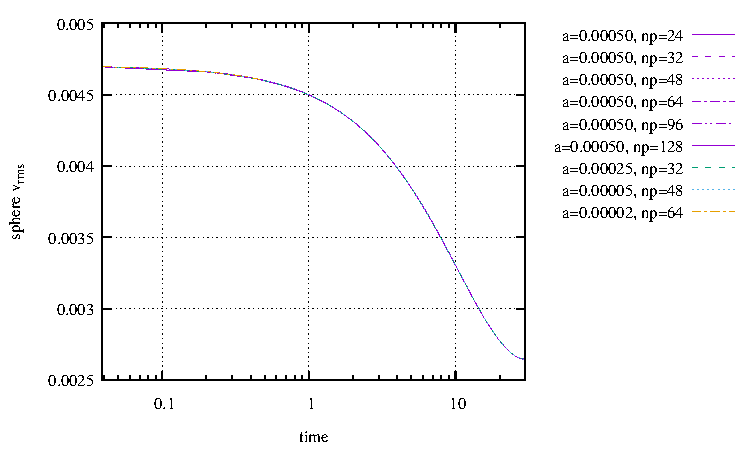
\includegraphics[width=5.7cm]{python_codes/fieldstone_93/results/vrms_sphere}
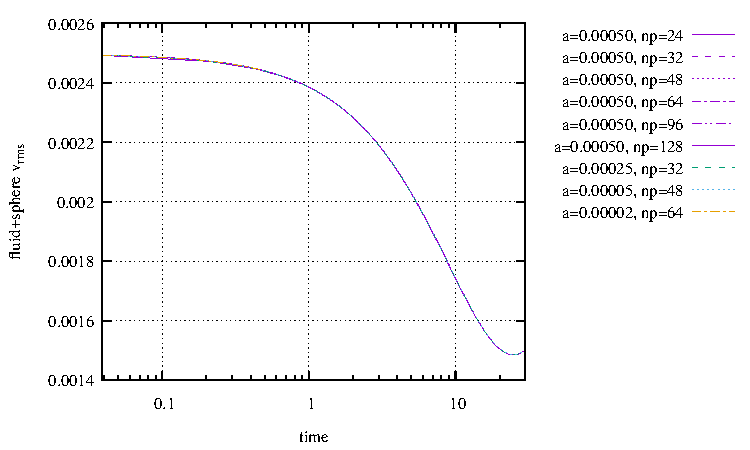
\includegraphics[width=5.7cm]{python_codes/fieldstone_93/results/vrms_fluidsphere}\\
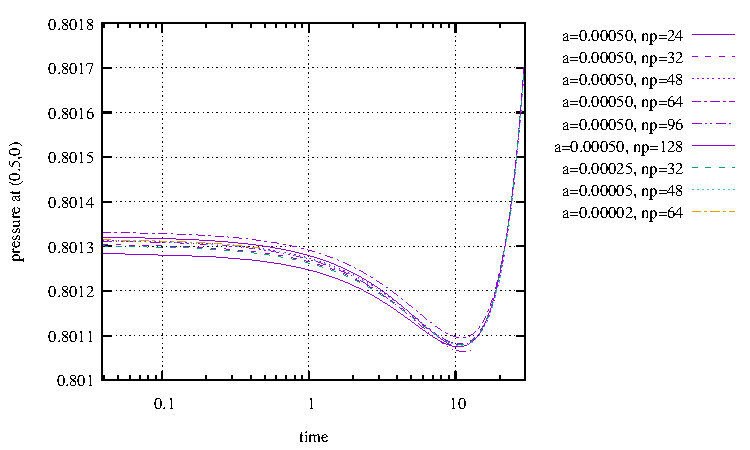
\includegraphics[width=7cm]{python_codes/fieldstone_93/results/p_bottom}
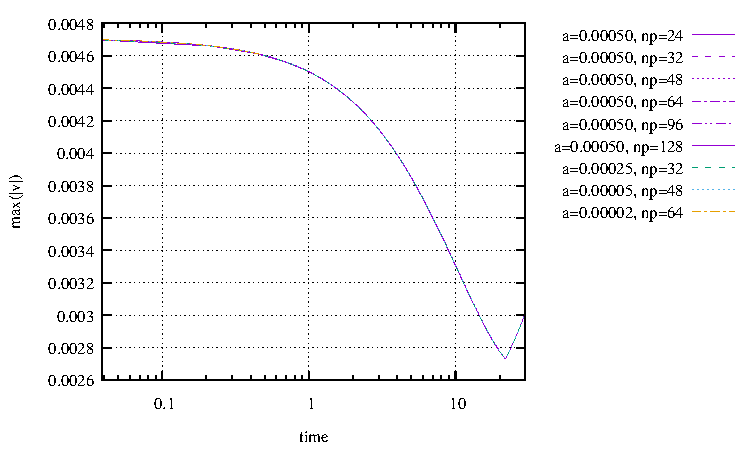
\includegraphics[width=7cm]{python_codes/fieldstone_93/results/max_vel}\\
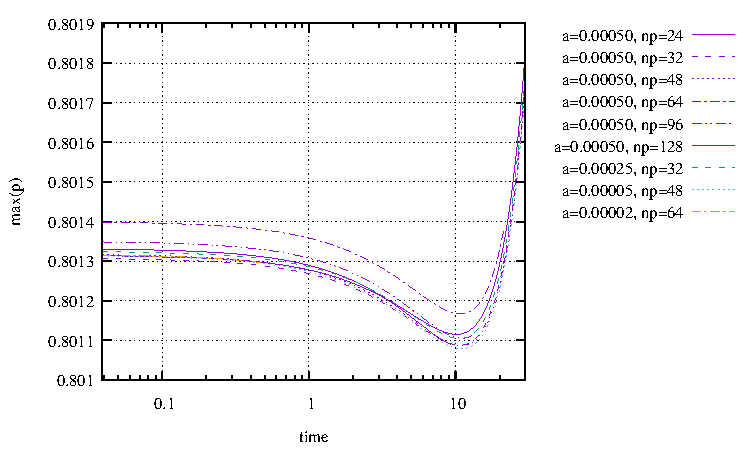
\includegraphics[width=5.7cm]{python_codes/fieldstone_93/results/max_press}
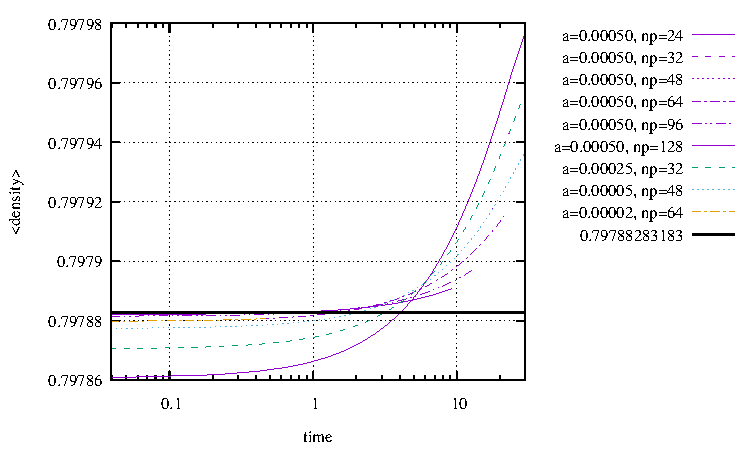
\includegraphics[width=5.7cm]{python_codes/fieldstone_93/results/avrg_density}
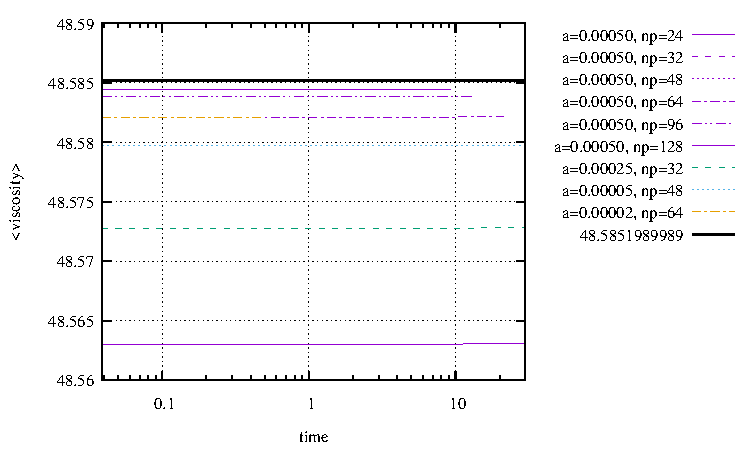
\includegraphics[width=5.7cm]{python_codes/fieldstone_93/results/avrg_viscosity}\\
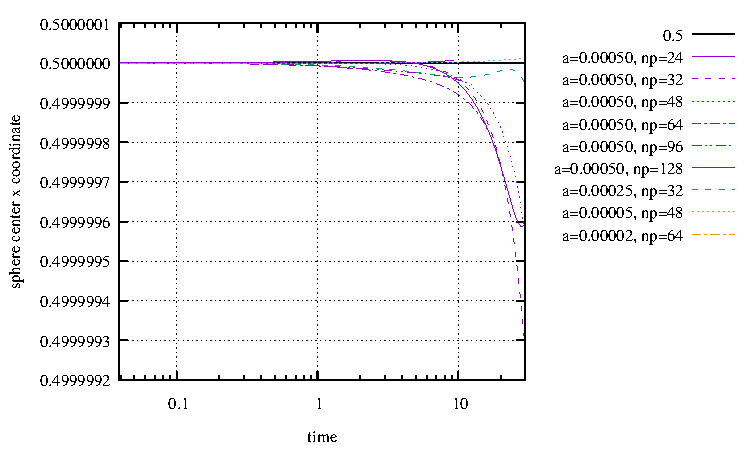
\includegraphics[width=7cm]{python_codes/fieldstone_93/results/center_position_x}
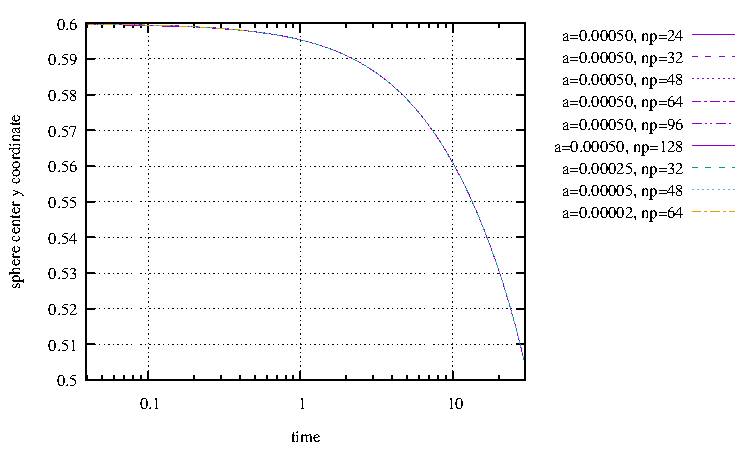
\includegraphics[width=7cm]{python_codes/fieldstone_93/results/center_position_y}\\
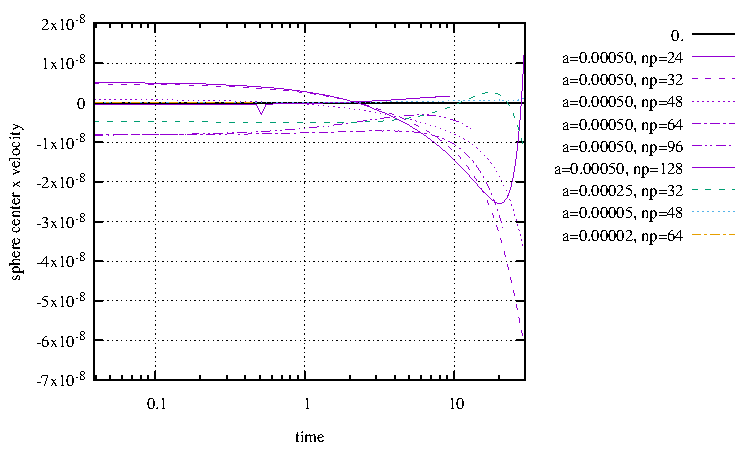
\includegraphics[width=7cm]{python_codes/fieldstone_93/results/center_velocity_x}
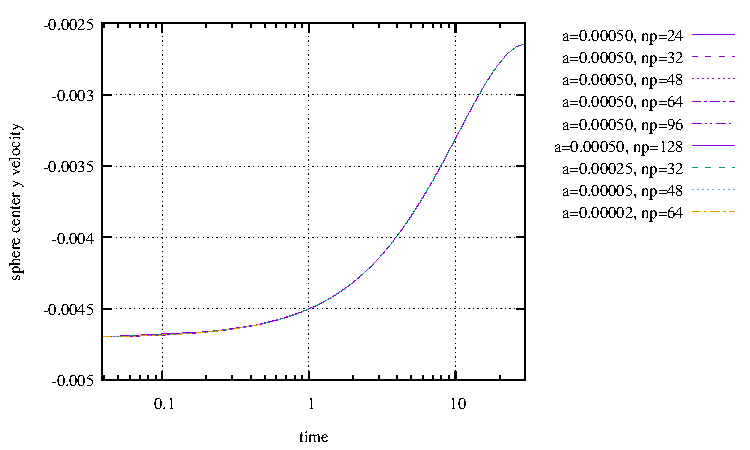
\includegraphics[width=7cm]{python_codes/fieldstone_93/results/center_velocity_y}\\
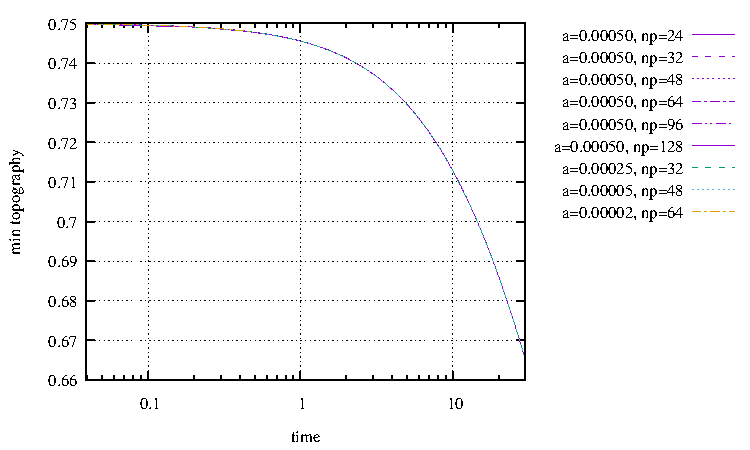
\includegraphics[width=7cm]{python_codes/fieldstone_93/results/topography_min}
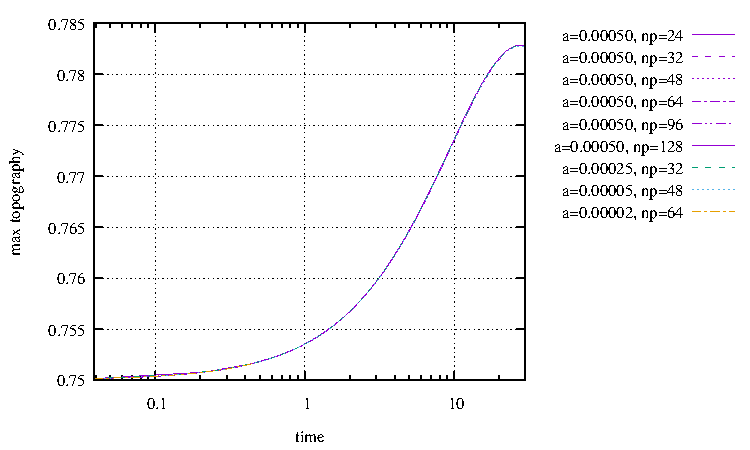
\includegraphics[width=7cm]{python_codes/fieldstone_93/results/topography_max}\\
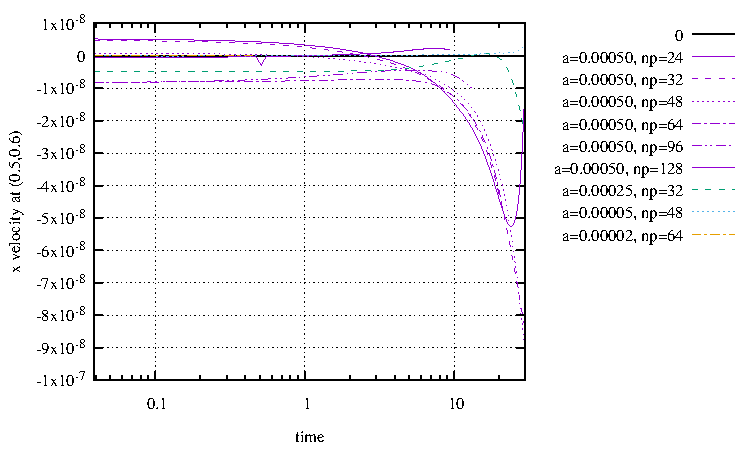
\includegraphics[width=5.7cm]{python_codes/fieldstone_93/results/point_u}
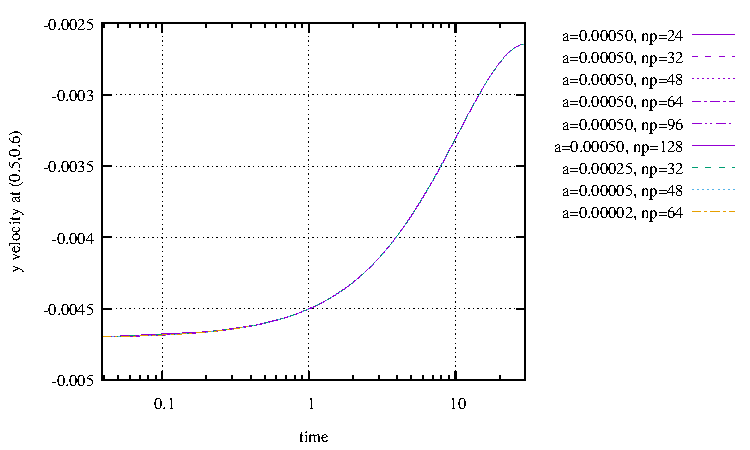
\includegraphics[width=5.7cm]{python_codes/fieldstone_93/results/point_v}
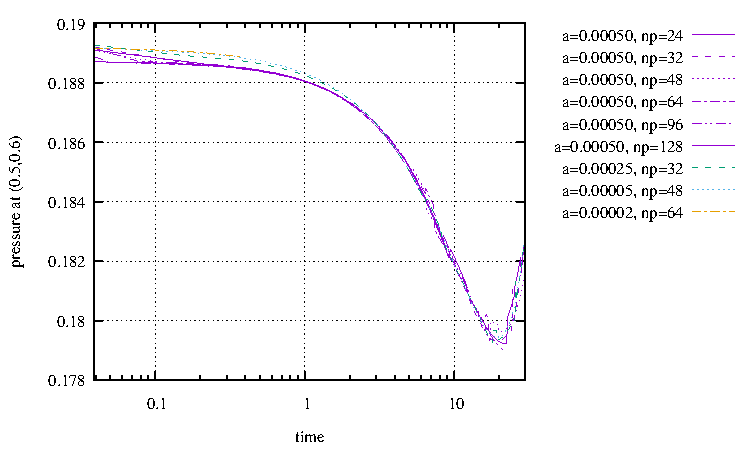
\includegraphics[width=5.7cm]{python_codes/fieldstone_93/results/point_p}\\
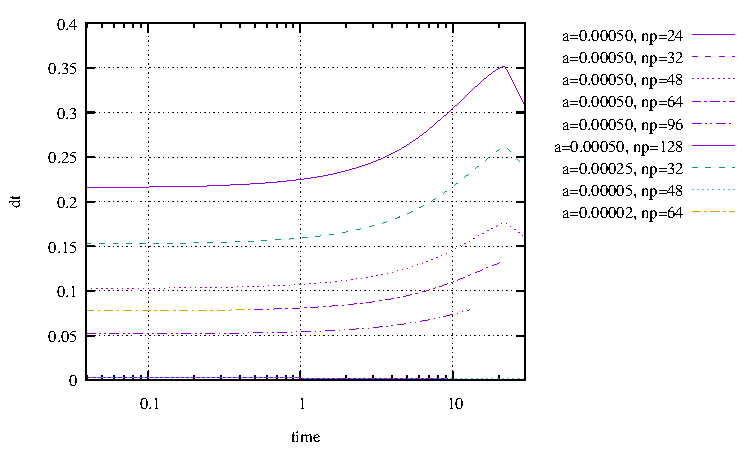
\includegraphics[width=5.7cm]{python_codes/fieldstone_93/results/dt}
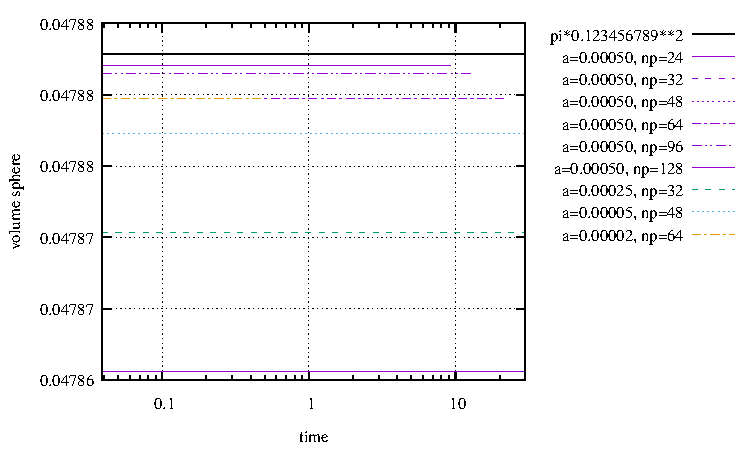
\includegraphics[width=5.7cm]{python_codes/fieldstone_93/results/vol_sphere}
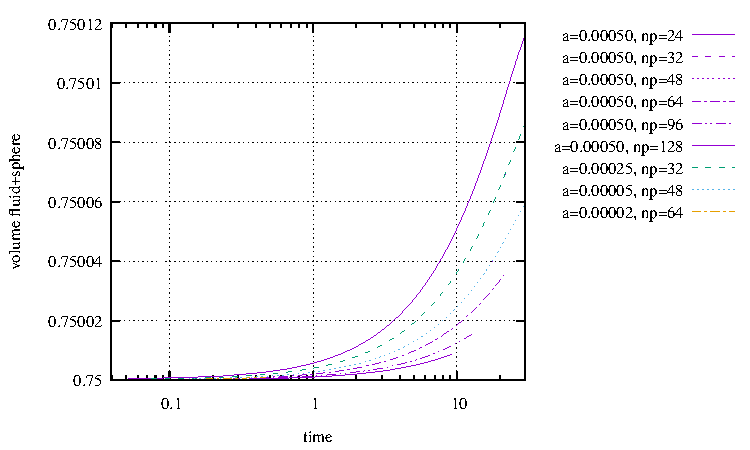
\includegraphics[width=5.7cm]{python_codes/fieldstone_93/results/vol_fluidsphere}
\end{center}

Results are remarkably similar for all resolutions. Note that because the pressure 
is discontinuous across element edges, the recorded value at (0.5,0.6) shows small
jumps.













